% coding:utf-8

%----------------------------------------
%FOSADSVB, a LaTeX-Code for a summary of digital signal processing
%Copyright (C) 2020, Thomas Annen

%This program is free software; you can redistribute it and/or
%modify it under the terms of the GNU General Public License
%as published by the Free Software Foundation; either version 2
%of the License, or (at your option) any later version.

%This program is distributed in the hope that it will be useful,
%but WITHOUT ANY WARRANTY; without even the implied warranty of
%MERCHANTABILITY or FITNESS FOR A PARTICULAR PURPOSE.  See the
%GNU General Public License for more details.
%----------------------------------------

\chapter{Neuronale Netze}
%===============================================================================
\section{Einführung}
Deep Learning ist eine Möglichkeit, Machine Learning Aufgaben umzusetzen. Folgende Varianten existieren: 
\begin{itemize}[noitemsep,topsep=3pt]
	\item Unsupervised: Finden von Mustern in Daten
	\item Supervised: Für einen neuen Input den Ausgang vorhersagen, basierend auf Beispielsdaten (Input/Output)
	\begin{itemize}[noitemsep]
		\item Regression: Bei der Ausgangsgrösse handelt es sich um echte Werte, z.B. Temperatur am nächsten Tag.
		\item Classification: Die Ausgangsgrössen werden mit Klassen gelabelt. 
	\end{itemize}
\end{itemize}
\begin{center}
		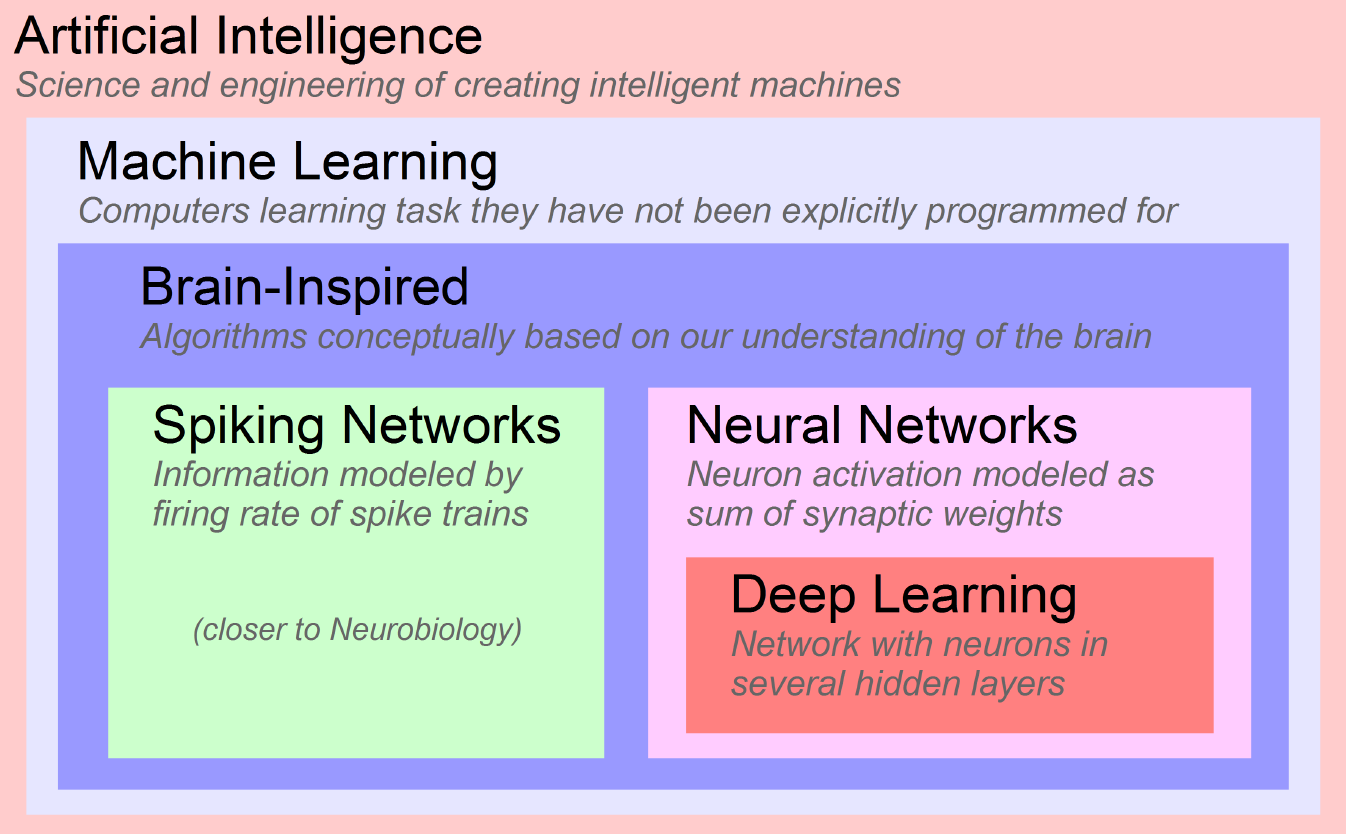
\includegraphics[width=0.6\textwidth]{../fig/ai_overview}
\end{center}
\subsection{Anwendungsgebiete}
\begin{itemize}[noitemsep,topsep=3pt]
	\item Objektklassifizierung/Detektion/Segmentierung
	\item Autonomes Fahren (Fahrzeuge)
	\item Geräuschunterdrückung in Echtzeit
	\item Automatisches Einfärben von schwarz/weiss Photos
\end{itemize}
\subsection{Gründe für Einsatz \& Popularität}
\begin{itemize}[noitemsep,topsep=3pt]
	\item Deep Learning liefert für spezifische Aufgaben bessere Resultate als der Mensch
	\item Probleme, die mathematisch nur schwer modelliert werden können, werden lösbar
	\item Vortrainierte Netzwerke sind verfügbar (transfer learning)
	\item Rechenleistung ist mittlerweile durch GPUs vorhanden
\end{itemize}
\subsection{Typen-Übersicht}
Weit verbreitete Strukturen sind das \emph{Convolutional Neural Network} (CNN) sowie das 
\emph{Deep Convolutional Network} (DCN), welches zu der Klasse der "'feedforward Netzwerke"'
gehört. Im Bereich der Spracherkennung und dem zeitlichen Verlauf von Daten sind 
\emph{Recurrent Neural Networks} (RNN), welche einen Feedback-Loop beinhalten.\\\\
CNN und RNN können mit FIR- und IIR-Filtern verglichen werden.
\newpage
\subsection{Vergleich: Nature vs. AI Networks}
\begin{itemize}[noitemsep,topsep=3pt]
	\item Das Menschliche Gehirn beinhaltet $\approx 8.6 \cdot 10^{10}$ Neuronen.
	\item Jedes Neuron ist durchschnittlich mit 7000 Synapsen mit anderen Neuronen verbunden.
	\item Die "'synaptic weights"' sind lernbar und beeinflussen die Funktionalität des Gehirns.
	\item AI Netzwerke modellieren den Ausgang von Neuronen als gewichtete Summe von Eingängen 
				und einer nicht-linearer Funktion. Diese nicht lineare Funktion wird "'Activation function"' 
				genannt, der Ausgang eines Neurons einfach nur "'Activation"'.
\end{itemize}
\begin{center}
		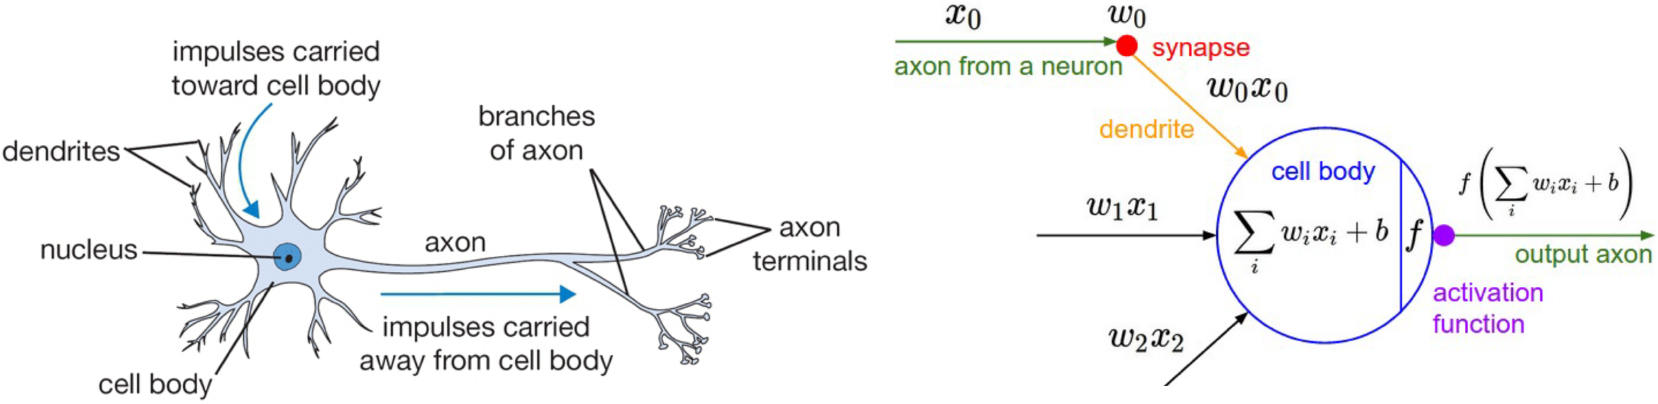
\includegraphics[width=0.75\textwidth]{../fig/neuron_aufbau}
\end{center}

%===============================================================================
\section{Prinzipielle Architektur für Bildklassifikation}
\begin{itemize}[noitemsep,topsep=3pt]
	\item Die Dimensionen eines Layers entsprechen der Anzahl Neuronen (Aktivierungen) am Layer-Ausgang.
	\item Die Anzahl Dimensionen des Eingangs-Layers entsprechen der Anzahl Pixel am Eingangsbild.
	\item Nach dem Eingangs-Layer führen mehrere Convolutional/Subsampling Layer die "'Feature Extraction"' durch.
	\item Aufeinanderfolgende "'fully connected layers"' führen die Klassifizierung durch.
	\item Die Anzahl Neuronen im Output Layer entspricht der Anzahl Klassen (Labels).
\end{itemize}
\begin{center}
		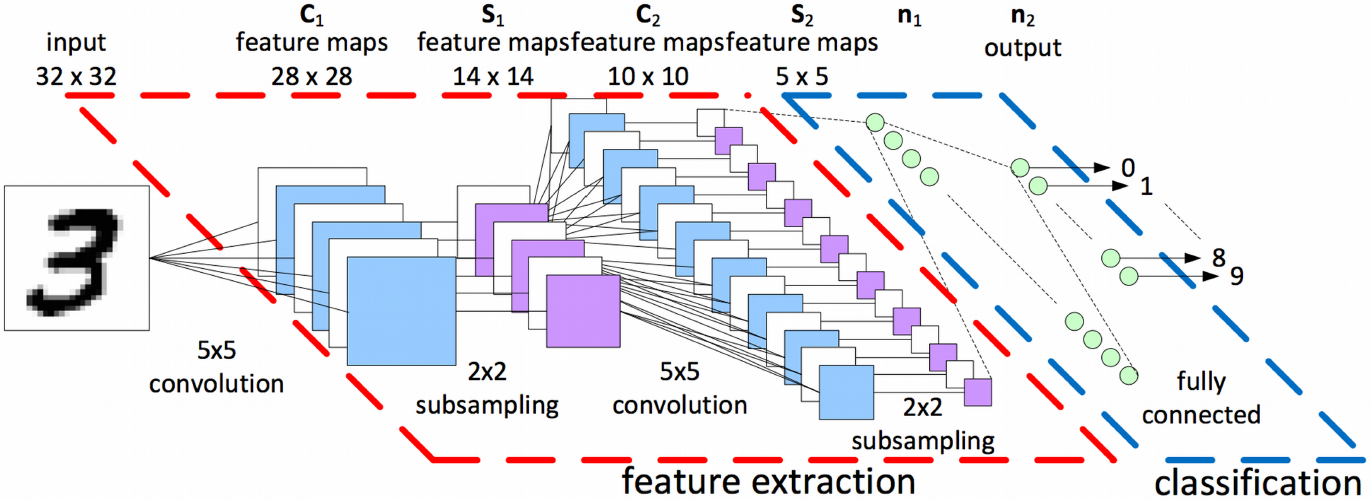
\includegraphics[width=0.8\textwidth]{../fig/cnn_architecture_image_recognition}
\end{center}

%===============================================================================
\section{Layer-Übersicht}
\subsection{Convolutional Layer}
Sind die fundamentalen Bauteile eines aktuellen DL neuronalen Netzwerkes. Eine Filtermaske
wird über das Bild gelegt und mit dem Input gefaltet (sliding window Verfahren). 
\begin{center}
		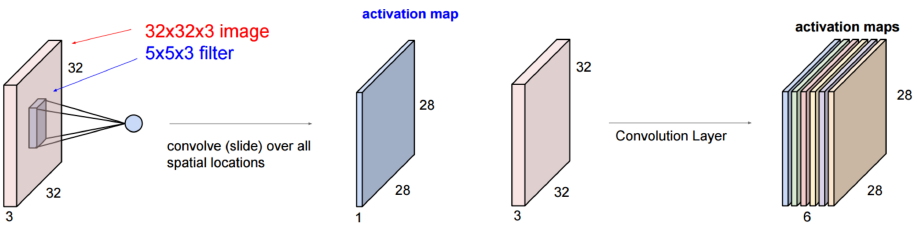
\includegraphics[width=0.8\textwidth]{../fig/convolutional_layer}
\end{center}
In jedem Schritt über die input feature map werden die Filterkoeffizienten mit dem unterliegenden Input elementweise multipliziert. Die Schrittgrösse nennt man "'stride"' und bestimmt die Ausgangs feature map, Grösse ($E$x$F$). Falls $R=S$ gilt, wird typischerweise eine Filtermaske mit der Grösse 1x1, 3x3, ... gewählt. 
\begin{center}
		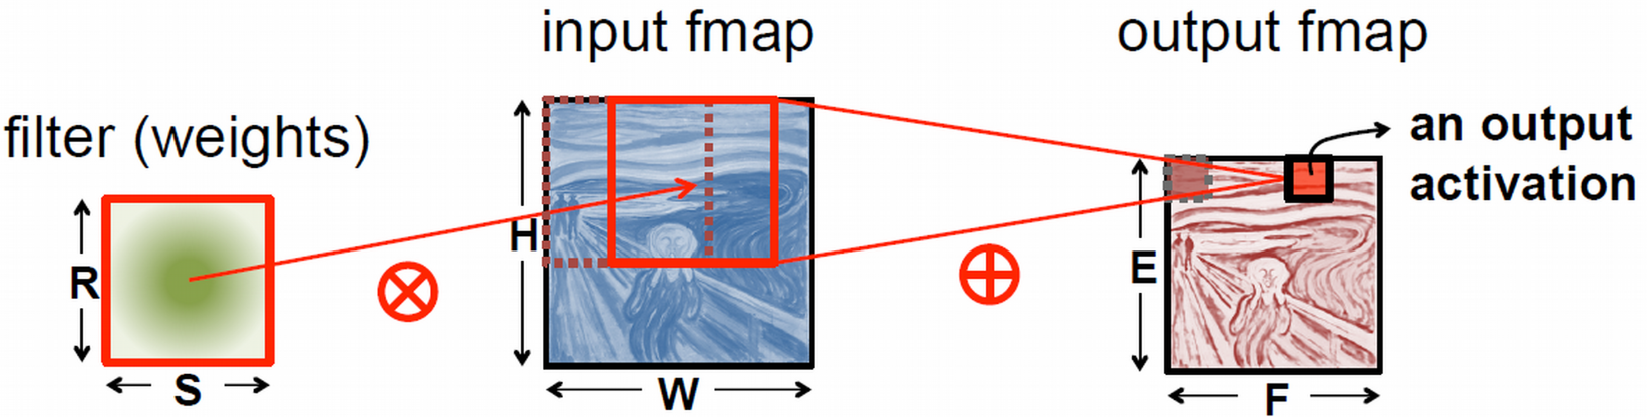
\includegraphics[width=0.45\textwidth]{../fig/convolutional_layer_details1}
\end{center}
Falls mehr als eine input feature map existiert, werden alle feature maps auf einmal mit einem 3D-Filterkernel berechnet. In jedem Convolutional Layer entspricht die Anzahl der input feature maps demnach der Anzahl der Filter Channels $C$. Typischerweise ist $1 \leq C \leq 128$. Nur am ersten Convolutional Layer ist typischerweise $C=1$, gegen Ende kann sie grösser werden. 
\vspace{-4mm}
\begin{center}
		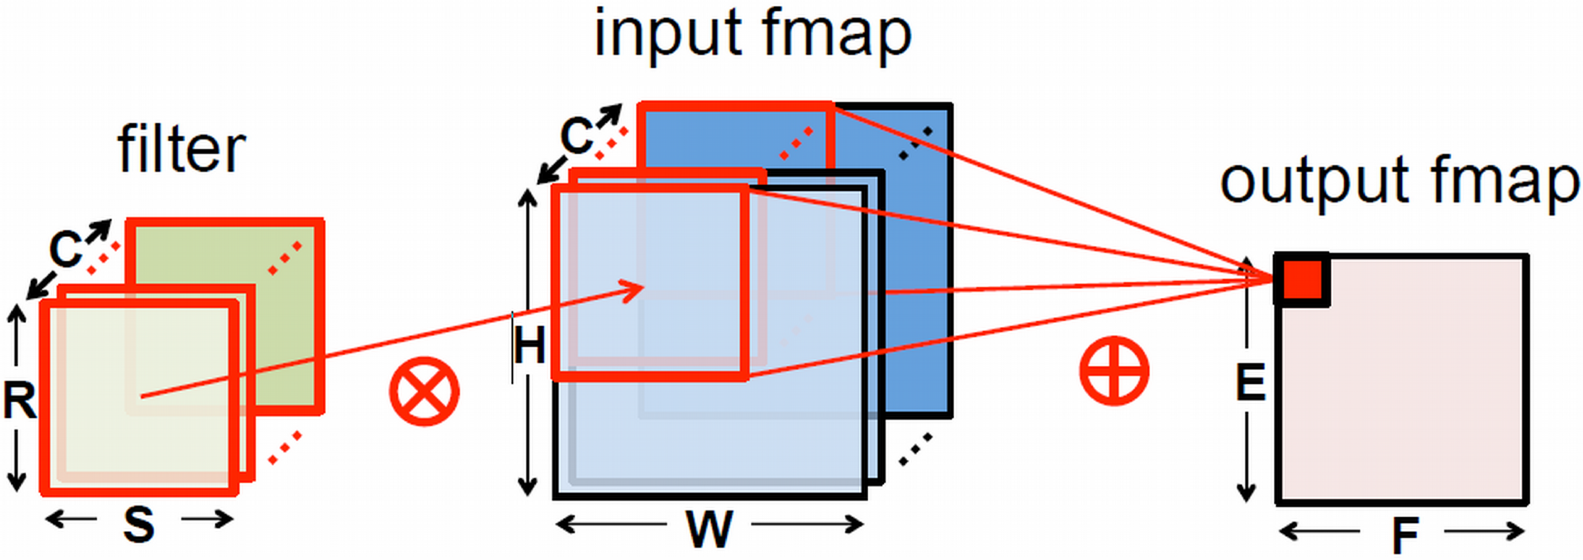
\includegraphics[width=0.35\textwidth]{../fig/convolutional_layer_details2}
\end{center}
Oft wird mehr als ein 3D-Filter pro Convolutional Layer angewendet. Wenn im $k$-ten Convolutional Layer $M$ Filter angewendet werden, dann entstehen aus den resultierenden  $M$ output feature maps von Layer $k$ schlussendlich $C$ input feature maps in Layer $k+1$.
\vspace{-4mm}
\begin{center}
		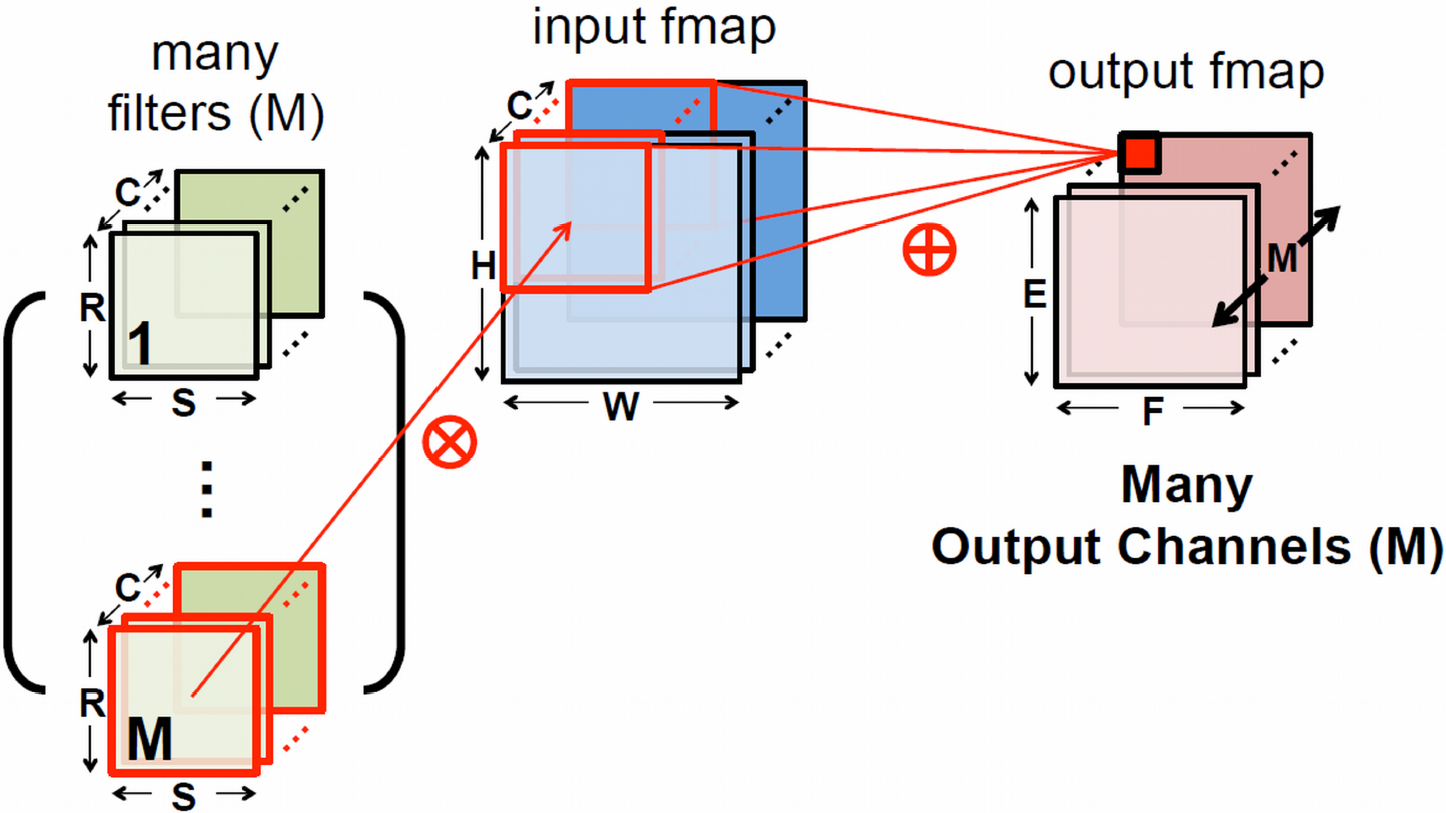
\includegraphics[width=0.4\textwidth]{../fig/convolutional_layer_details3}
\end{center}
Falls $N>1$, spricht man von "'batch processing"', es wird also mehr als ein Bild auf einmal durch das Netzwerk verarbeitet. 
\vspace{-4mm}
\begin{center}
		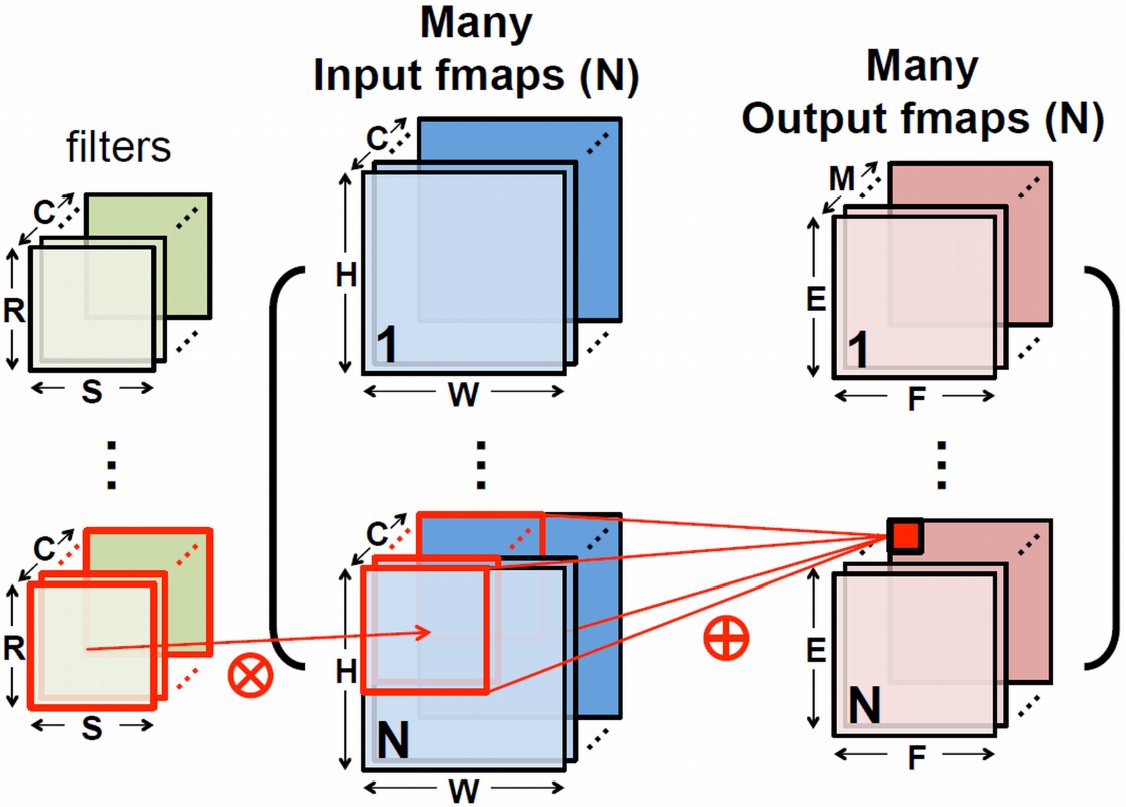
\includegraphics[width=0.375\textwidth]{../fig/convolutional_layer_details4}
\end{center}
Die unten ersichtlichen Formeln gehen davon aus, dass kein Padding am Eingang durchgeführt wird.
\begin{align*} 
	\text{\textbf{O}}[n][m][x][y] = \text{Activation}\bigg( \text{\textbf{B}}[m] + \sum_{i=0}^{R-1} \sum_{j=0}^{S-1} \sum_{k=0}^{C-1} \text{\textbf{I}}[n][k][Ux+i][Uy+j] \times \text{\textbf{W}}[m][k][i][j] \bigg), \\
	0\leq n < N, 0\leq m < M, 0\leq y < E, 0 \leq x <F,\\
	E=(H-R+U)/U,F=(W-S+U)/U
\end{align*}
\begin{center}
		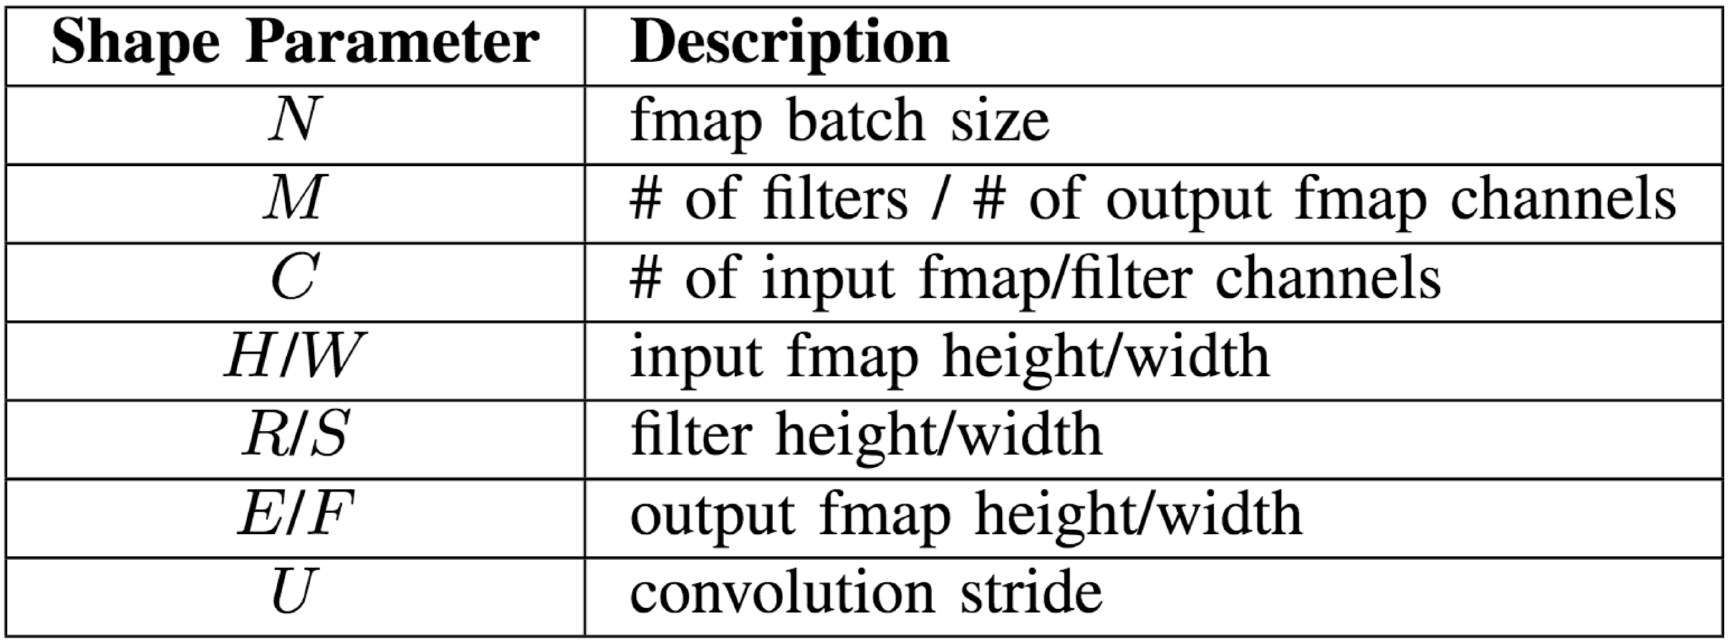
\includegraphics[width=0.45\textwidth]{../fig/naming_cnn}
\end{center}
\subsection{Pooling Layer}
Werden zwischen Convolutional Layers platziert. Beim Pooling wird die Tiefe beibehalten, 
es findet aber ein Downsampling für Breite \& Höhe statt. Der zugehörige Faktor nennt 
sich "'stride"'. Das Pooling reduziert die Anzahl Gewichte welche trainiert werden müssen 
und somit den Rechenaufwand. 
\begin{center}
		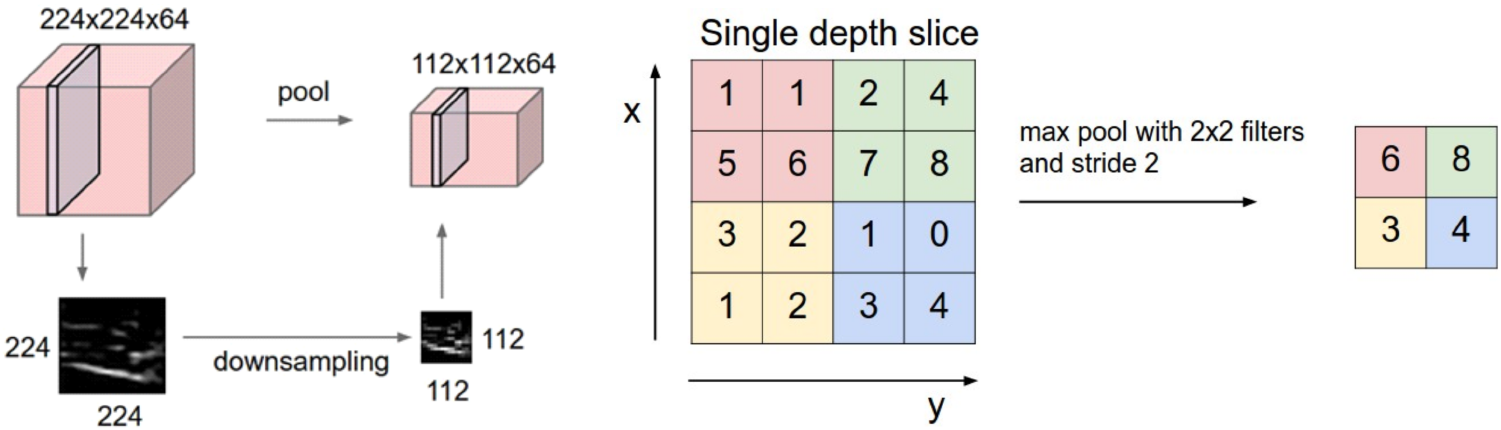
\includegraphics[width=0.8\textwidth]{../fig/pooling_layer}
\end{center}
\subsection{Activation Layer}
Repräsentiert eine nicht-lineare Operation in der Übertragungsfunktion eines Neurons. 
Es existieren verschiedene Funktionen, die ReLu-Funktion ist am weitesten verbreitet. 
\begin{center}
		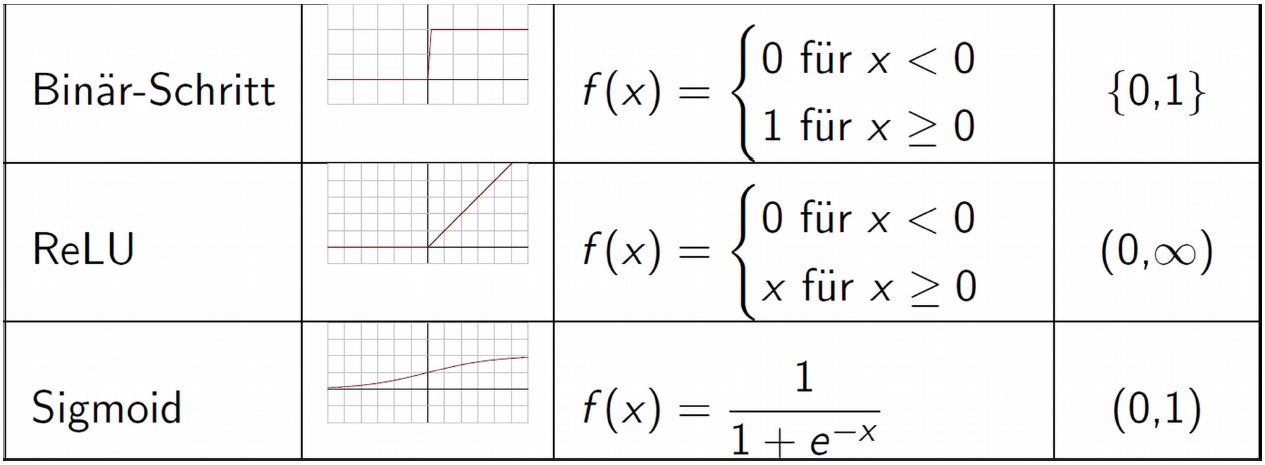
\includegraphics[width=0.40\textwidth]{../fig/activation_layer}
\end{center}

%===============================================================================
\section{Layer-Entwicklung}
\textbf{Begriffserläuterung:}
\begin{itemize}[noitemsep,topsep=3pt]
	\item Padding: Ergänzen der Daten am Rand, damit die ganze Filtermaske im Bild Platz findet.
\end{itemize}
\textbf{Filtergrössen:}
Die Filergrössen sind entscheidend für die Qualität, Speicherbedarf sowie Rechendauer.
\begin{itemize}[noitemsep,topsep=3pt]
	\item Pooling jeweils mit (2x2) Filter (stride = 2), Fully Connect mit 10 Ausgangsklassen
	\item Layer 2 (Conv 1) enthält 8 (3x3) Filter
	\item Layer 6 (Conv 2) enthält 16 (3x3) Filter
	\item Layer 10 (Conv 3) enthält 32 (3x3) Filter
\end{itemize}

\begin{center}
		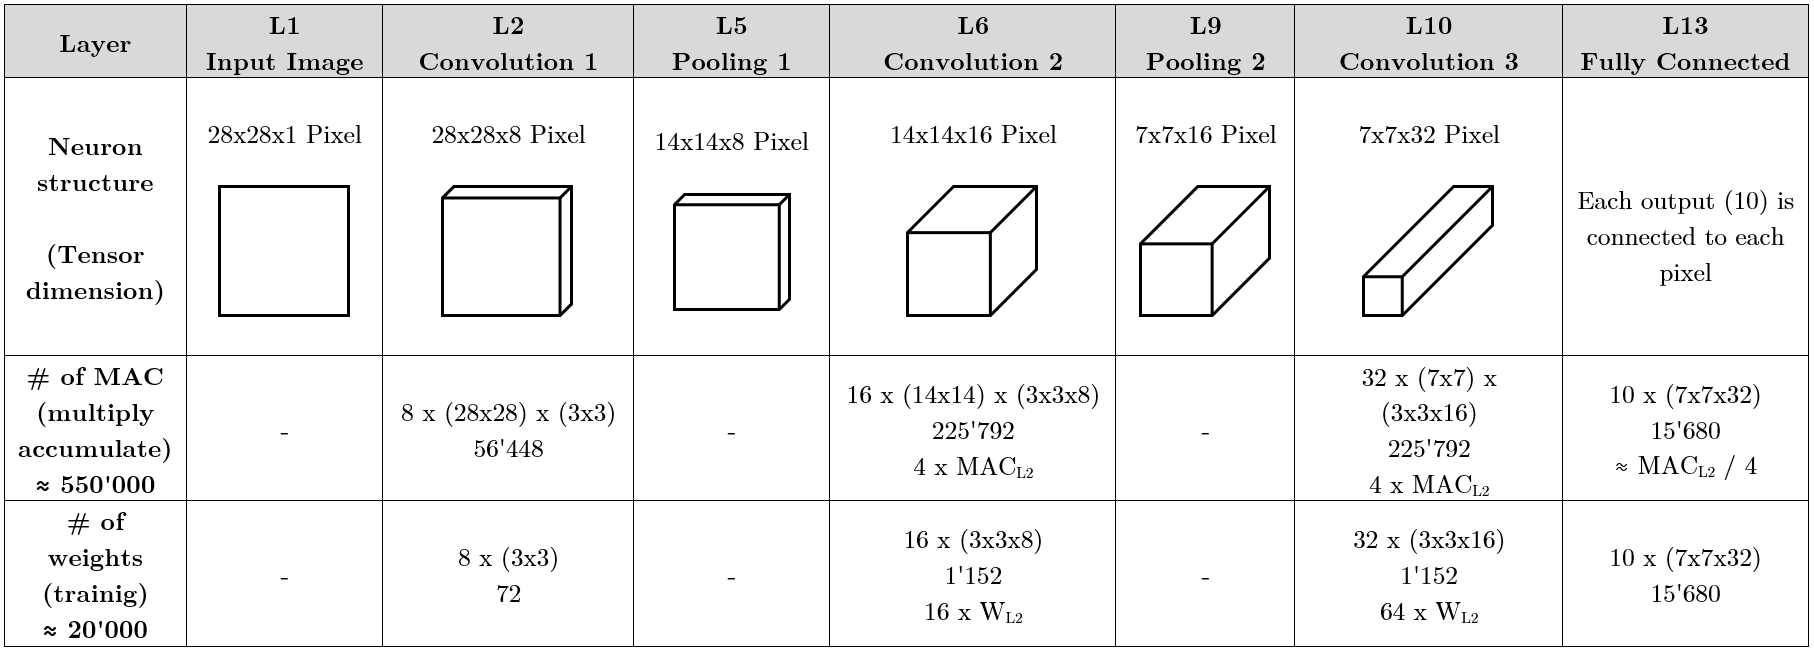
\includegraphics[width=\textwidth]{../fig/cnn_overview}
\end{center}
Fazit: Faltung benötigt zur Laufzeit viel Rechenzeit, Training generiert die Gewichtungen 
und benötigt deshalb Speicher. Der Zugriff auf die extern gespeicherten Gewichtungen ist 
dabei Energieintensiv. 

